% !TEX root = Tesi.tex
\chead{}

\chapter{From models to code, a case study.}

This chapter covers a case study based on the applications of the notions previously retrieved describing the Magento platform the Madison Island eCommerce website would run on and proposing a possible automation for code generation compatible with the platform ecosystem and architecture.

\section{Magento eCommerce Platform}

Magento is one of the most powerful and feature-rich online eCommerce platform that was launched on March 31, 2008. 

The platform grants merchants complete flexibility and control over the look, content and functionality of their online store. Thanks to its intuitive administration interface for content management and robust marketing and merchandising tools it gives merchants the ability to create sites that are fully fit their unique business needs, putting no constraints on business processes and flow.

From a technical perspective, the platform incorporates the core architectural principles of an object-oriented, PHP-based application that can be easily used to personalize and expand the existing and already ample out of the box set of features.
In fact, central to the Magento model of software development is the strategy of replacing or extending core code rather than editing it to support maintainability and flexibility. 

To achieve this goal Magento software architecture has been built around the concept of self-contained modules holding discrete code organized by feature, thereby reducing each module’s external dependencies.

The Magento frontend is designed to optimize storefront customization, with highly extensible themes being the central customization mechanism so that merchants can easily extend and transform the appearance of their storefronts.



\vspace{0.5cm}
\begin{figure}[H]
  \centering
    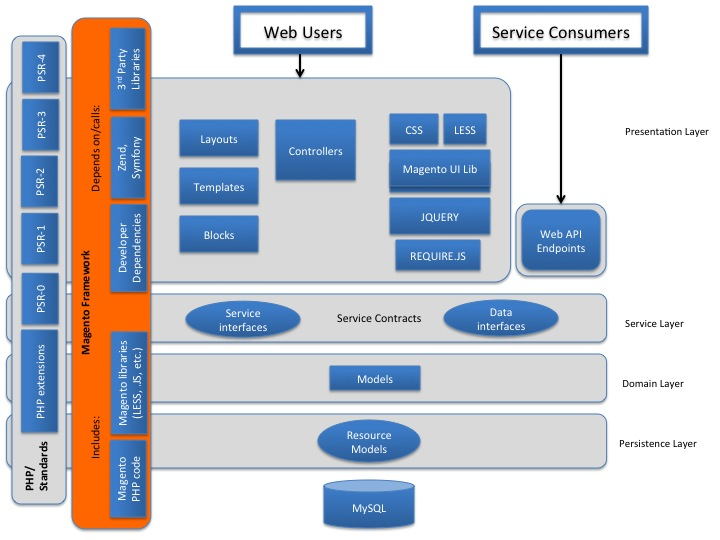
\includegraphics[height=12cm]{images/magento-architecture.jpg}
  \caption{Magento Architecture Overview}
  \label{fig:magento-architecture-overview}
\end{figure}
\vspace{0.5cm}


Interacting with the product and its appearance on a Magento web interface means interacting with presentation layer code composed by both view elements (layouts, blocks, templates) and controllers, which process commands to and from the user interface. 

We can extensively customize this user interface by extending Magento themes capabilities personalizing its content modifying this presentational layer accordingly to the requirements because the theme is responsible for organizing both the visual aspect of the interface and the product behavior.

Each Magento theme resides in a specific directory and includes custom page layouts, templates, skins, and language files that work together to create a distinct user experience.

In our case study example, the Madison Island frontend is built around the technology that we just described using a personalized and customized Magento theme for the user experience on the website. Specifically, each page of the website can be thought as a composition of Magento blocks representing a specific page layout tree that get assembled and internally rendered before being returned to the user. As shown in \ref{fig:madison-island-magento-theme-overview} each one of these blocks holds its associated rendering template and this is how the final output is composed.

\vspace{0.5cm}
\begin{figure}[H]
  \centering
    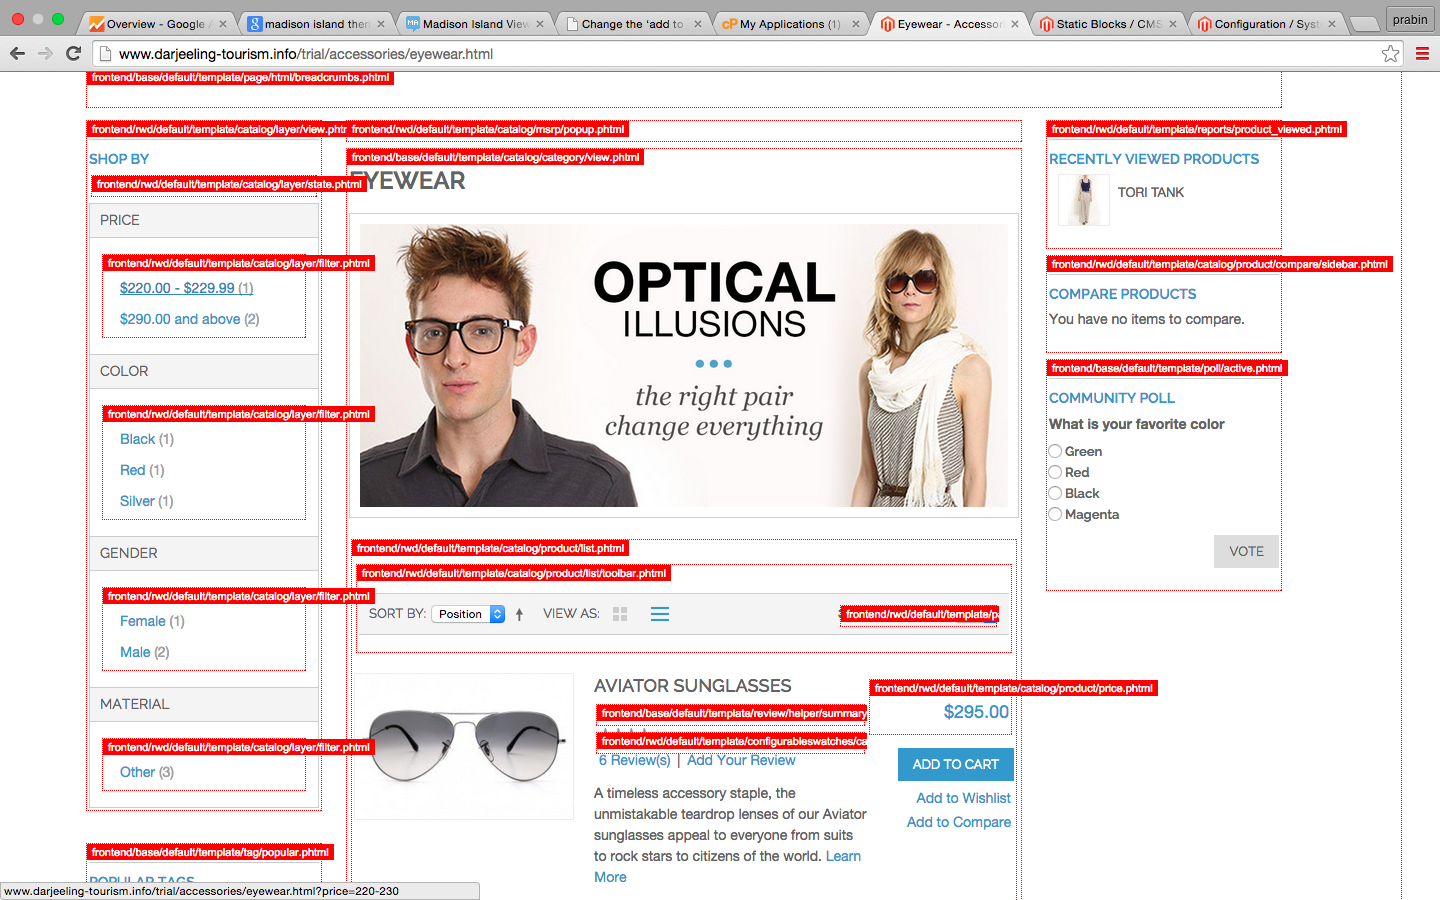
\includegraphics[height=10cm]{images/madison-island-theme.png}
  \caption{Madison Island Magento Theme Overview}
  \label{fig:madison-island-magento-theme-overview}
\end{figure}
\vspace{0.5cm}





\section{Serializing Models}

\section{Magento extension}


%\addcontentsline{toc}{chapter}{}
